
% --- SLIDE 1 ---
\begin{frame}{Wprowadzenie - czym są dane osobowe?}
    \begin{alertblock}{Dlaczego dane osobowe są istotne?}
      \begin{itemize}
        \item Dane osobowe to informacje umożliwiające identyfikację osoby fizycznej.\cite{PII_USDE}
        \item W Internecie udostępniamy je świadomie i nieświadomie.
        \item Ich analiza pozwala tworzyć dokładne profile użytkowników.
      \end{itemize}
    \end{alertblock}
  \end{frame}
  
  % --- SLIDE 2 ---
  \begin{frame}{Dane jawnie udostępniane}
  \begin{columns}[c]
      \column{.5\textwidth}
      \begin{alertblock}{Co użytkownicy podają sami?}
        \begin{itemize}
          \item Nazwa użytkownika, zdjęcie profilowe, data urodzenia
          \item Posty, komentarze, aktywność na forach
          \item Informacje udostępniane podczas zakupów lub rejestracji - od imienia i nazwiska, po adres zamieszkania.\cite{CYB_DEF_NAJCZĘSTRZE_DANE}
        \end{itemize}
      \end{alertblock}
      \column{.5\textwidth}
      \begin{figure}
        \centering
        
\includegraphics[height=0.45\textheight]{images/social-media.png}
        \label{fig:social-media}
      \end{figure}
  \end{columns}
  \end{frame}
  
  % --- SLIDE 3 ---
  \begin{frame}{Dane techniczne i ukryte}
  \begin{columns}[c]
      \column{.5\textwidth}
      \begin{figure}
        \centering
        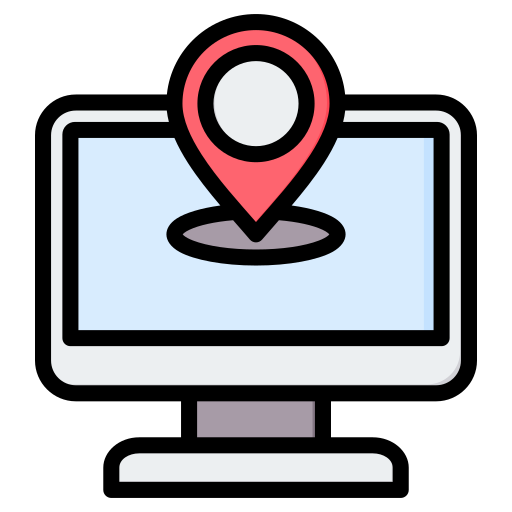
\includegraphics[height=0.45\textheight]{images/ip-address.png}
        \label{fig:ipTracking}
      \end{figure}
      \column{.5\textwidth}
      \begin{alertblock}{Co zbierane jest w tle?}
        \begin{itemize}
          \item Adres IP, nagłówki HTTP, czas trwania sesji
          \item Fingerprinting urządzenia - unikalna konfiguracja przeglądarki
          \item Pliki cookies i śledzenie międzystronowe
        \end{itemize}
      \end{alertblock}
  \end{columns}
  \end{frame}
  
  % --- SLIDE 4 ---
  \begin{frame}{Dane jednoznacznie identyfikujące}
    \begin{alertblock}{Informacje bezpośrednio wskazujące osobę}
      \begin{itemize}
        \item Numer PESEL, numer telefonu, adres e-mail
        \item Informacje z dokumentów tożsamości
        \item Zbiory danych, które zawierają dane jawne \cite{LEXDIGITAL_CZY_IMIE_NAZW_TO_DANE_OS}
      \end{itemize}
    \end{alertblock}
  \end{frame}
  
  % --- SLIDE 5 ---
  \begin{frame}{Dane quasi-identyfikujące}
  \begin{columns}[c]
      \column{.5\textwidth}
      \begin{alertblock}{Dane, które ujawniają więcej niż myślisz}
        \begin{itemize}
          \item Kod pocztowy, wiek, płeć
          \item Łącznie mogą jednoznacznie wskazać osobę
          \item Przykład: 87\% Amerykanów możliwych do identyfikacji na podstawie 3 zmiennych
        \end{itemize}
      \end{alertblock}
      \column{.5\textwidth}
      \begin{figure}
        \centering
        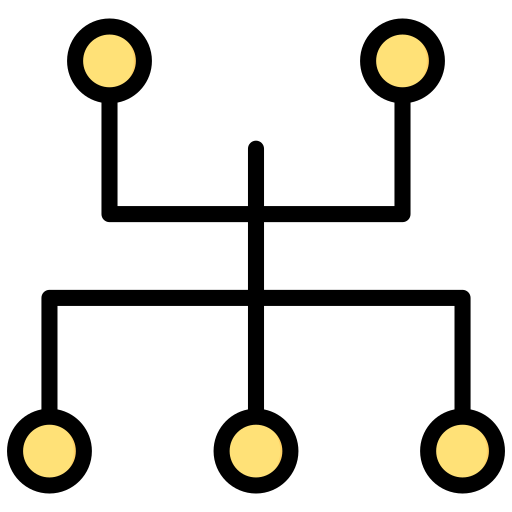
\includegraphics[height=0.45\textheight]{images/network-topology.png}
        \label{fig:quasiIdentifiers}
      \end{figure}
  \end{columns}
  \end{frame}
  
  % --- SLIDE 6 ---
  \begin{frame}{Identyfikacja przez korelację danych}
  \begin{columns}[c]
      \column{.5\textwidth}
      \begin{figure}
        \centering
        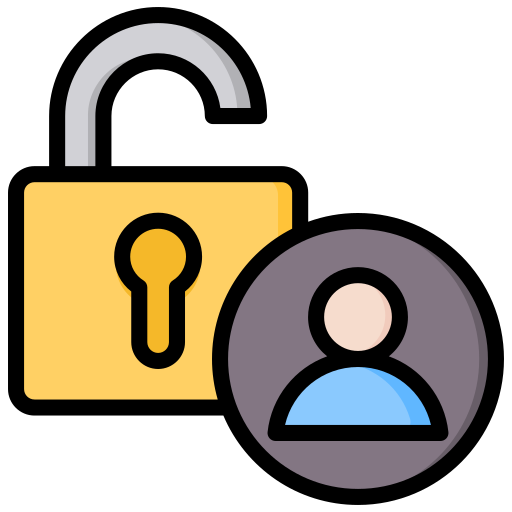
\includegraphics[height=0.45\textheight]{images/access-control.png}
        \label{fig:dataCorrelation}
      \end{figure}
      \column{.5\textwidth}
      \begin{alertblock}{Łączenie pozornie nieszkodliwych danych}
        \begin{itemize}
          \item Łączenie różnych zbiorów danych zwiększa ryzyko deanonimizacji
          \item Przykład: dane z forów + metadane przeglądarki = pełna identyfikacja
          \item Dane z różnych źródeł mogą „dopełnić” profil
        \end{itemize}
      \end{alertblock}
  \end{columns}
  \end{frame}
  
  % --- SLIDE 7 ---
  \begin{frame}{Dane biometryczne i behawioralne}
    \begin{alertblock}{Jak zachowanie nas zdradza?}
      \begin{itemize}
        \item Głos, odciski palców, sposób chodzenia, rozpoznawanie twarzy
        \item Styl pisania, rytm korzystania z klawiatury/myszy
        \item Dane zbierane przez urządzenia i aplikacje mobilne
      \end{itemize}
    \end{alertblock}
  \end{frame}
  
  % --- SLIDE 8 ---
  \begin{frame}{Case study: identyfikacja w badaniach DNA}
  \begin{columns}[c]
      \column{.5\textwidth}
      \begin{alertblock}{Czy dane genetyczne są naprawdę anonimowe?}
        \begin{itemize}
          \item Dane z publicznych baz (GEDmatch) wykorzystane do identyfikacji anonimowych uczestników badań DNA
          \item Połączenie danych genetycznych z metadanymi (wiek, miejsce) wystarczyło do identyfikacji 241 z 579 wybranych osób.\cite{DNA_LEAK}
        \end{itemize}
      \end{alertblock}
      \column{.5\textwidth}
      \begin{figure}
        \centering
        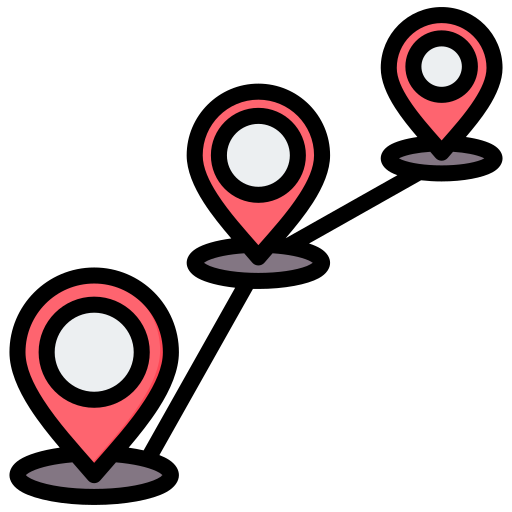
\includegraphics[height=0.45\textheight]{images/routing.png}
        \label{fig:dnaCase}
      \end{figure}
  \end{columns}=
  \end{frame}
  
  % --- SLIDE 9 ---
  \begin{frame}{Jak wiele ujawniamy?}
    \begin{alertblock}{Dlaczego warto wiedzieć, co udostępniamy?}
      \begin{itemize}
        \item Nawet pozornie nieszkodliwe dane mogą prowadzić do identyfikacji
        \item Nasza aktywność tworzy cyfrowy odcisk palca
        \item Im więcej danych - tym dokładniejszy profil
      \end{itemize}
    \end{alertblock}
  \end{frame}